\section{Development environment and simulation}
\label{sec:devenv}
During the process of developing the application, it became necessary to be able to continuously deploy and test the latest version without having to depend on flying the physical vehicle but instead relying on the simulation of the system inside the computer that was at the same time running the developed software.
This configuration has the twofold advantage of reducing the development time on the one hand since there is no need to be concerned with the interactions between the different hardware components, and the results can be visualized immediately on the computer screen, and on the other hand, of increasing the safety of the process by executing on the vehicle only software that has already been tested to an acceptable point.

Simulators allow PX4 flight code to control a computer-modelled vehicle in a simulated "world" that can be interacted with in the same ways as with an actual vehicle, using QGroundControl, an offboard API or a radio controller.
PX4 supports two different simulation modes: software-in-the-loop (SITL), where the flight stack runs on a non-dedicated computer, and hardware-in-the-loop (HITL), where the simulation firmware executes on an actual flight controller board.
Communication into and out of the flight stack uses the MAVLink protocol mentioned in section \ref{subsec:mavlink},
which allows exchanging messages between drones, ground control stations, and other MAVLink systems \cite{mavlink}.
When the firmware is simulated, a MAVLink server is always started as part of the running software to enable communication with the simulator program, and any other offboard entry point that could be present.


\begin{figure}
  \centering
  
\includegraphics[width=\textwidth,keepaspectratio]{img/px4_simulator_messages.png}
  \caption{MAVLink messages exchanged between the simulator and the flight stack during simulation.}
  \source{Adapted from \citetitle{px4-guide} \cite{px4-guide}.}
  \label{fig:simulator-msgs}
\end{figure}

In both SITL and HITL modes, the simulation works according to the feedback loop shown in figure~\ref{fig:simulator-msgs}. 
The simulator generates the input from the sensors based on its internal world representation and sends it through MAVLink messages to the flight stack running on the same computer using the UDP transport protocol.
This, in turn, generates response actuator controls that are fed back into the simulator in the same way to affect the vehicle's position, velocity, and attitude in the simulated world.
Simulated communications employ MAVLink messages specific to the mode in use and are not precisely the same as those used during non-simulated flights.

There are many options for simulators supported by PX4, like Gazebo, a robust 3D simulation environment for Linux systems that is particularly suited for testing object avoidance and is commonly used with ROS, or AirSim (\ref{subsec:airsim}), a more resource-intensive cross-platform simulator that leverages the Unreal Engine, typically used for game development and animation, to provide physically and visually realistic simulations.
For this project, AirSim was chosen because of previous experience with Unreal Engine, the easy availability of visual packages to test computer vision features and its native support for running on Windows machines, which is the operating system running on the computer where the tests will take place.
AirSim offers a library called \texttt{airlib} (\footnote{\url{https://pypi.org/project/airsim/}}), available for Python, that can be used to retrieve images taken from a simulated camera from the perspective of the drone in the simulation world.
This feature will be necessary when testing the person-recognition utilities used in the program.

\begin{figure}
  \centering
  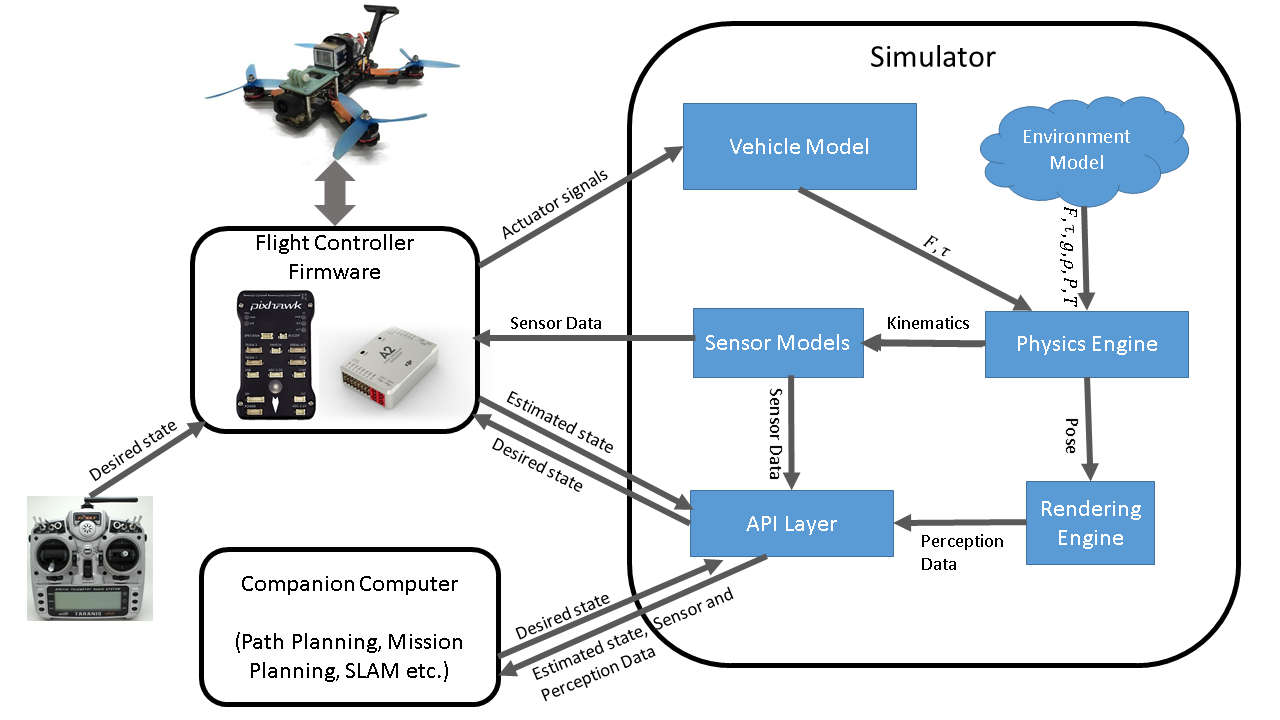
\includegraphics[width=\textwidth,keepaspectratio]{img/airsim-overview.png}
  \caption{High-level overview of how different components interact in the AirSim simulator.}
  \source{Adapted from \citetitle{airsim-paper} \cite{airsim-paper}.}
  \label{fig:airsim-overview}
\end{figure}

A high-level overview of the simulator architecture and how different components interact can be seen in figure \ref{fig:airsim-overview}. 
The API layer in the figure inside the simulator environment refers to AirSim's own \texttt{airlib} library, which exposes high-level functionality to send control commands to the flight controller directly.
However, in order to share the same control code between simulated flight and actual flight without depending on the simulator system, the control commands are sent using the official MavSDK API instead, which allows communication of estimated state, desired state and sensor data directly between the flight controller firmware and any connected systems.

In order to run the software-in-the-loop simulation, the PX4 firmware needs to be built from the source code on the Linux platform where it will run.
The build system then sets up all the necessary ports for the MAVLink communication and starts a local instance of the NuttX operating system that would run on the actual flight board.

\begin{figure}
  \centering
  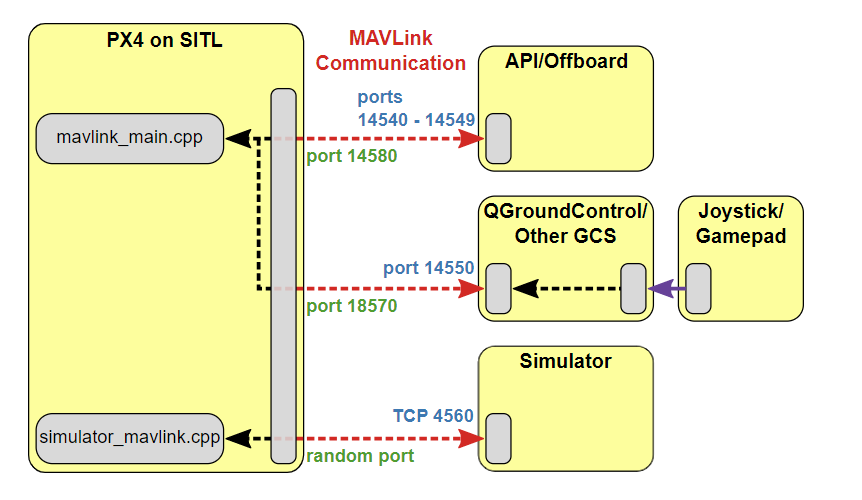
\includegraphics[width=\textwidth,keepaspectratio]{img/px4-ports.png}
  \caption{Network diagram between the components interconnecting during software-in-the-loop simulation.}
  \source{Adapted from \citetitle{px4-guide} \cite{px4-guide}.}
  \label{fig:px4-ports}
\end{figure}

Figure \ref{fig:px4-ports} shows how the different parts of the system communicate with each other inside a SITL simulation.
PX4 uses commonly established UDP ports for MAVLink communication with ground control stations (e.g. QGroundControl), offboard APIs (e.g. MAVSDK, MAVROS) and simulator APIs (e.g. AirSim, Gazebo).
Externally developed applications like Dronecontrol use an offboard API, in this case, MAVSDK, and therefore listen to PX4's remote UDP port 14540 by default.
All ports in the range 14540-14549 can be used to connect offboard APIs, for example, when controlling multiple vehicles simultaneously.
PX4's remote UDP Port 14550 is used for communication with ground control stations, which are expected to listen for connections on this port. QGroundControl listens to this port by default but can be configured to use the others, the same way offboard APIs can use the default ground station port to connect instead.
PX4 uses a simulation-specific module to connect to the simulator's local TCP port 4560.
Simulators then exchange information with PX4 using the Simulator MAVLink API shown in figure \ref{fig:simulator-msgs}. 
PX4 on SITL and the simulator can run either on the same computer or different computers on the same network \cite{px4-simulation}. (https://docs.px4.io/v1.12/en/simulation/)
\todo

Since one of the purposes of using AirSim as a simulator is to run it on a Windows computer and the PX4 software-in-the-loop stack runs best on Linux, it is necessary to run a virtualized Linux OS in parallel on the Windows computer and set up a local network so that the simulator and the flight controller firmware can communicate with each other.
The PX4 development team officially supports running the SITL flight stack in Windows through the Windows Subsystem for Linux (WSL2)\footnote{\url{https://docs.microsoft.com/en-us/windows/wsl/about}}, which allows users to install and run their Ubuntu Development Environment on Windows as if it was running it on a Linux computer.
The Windows Subsystem for Linux lets developers run a GNU/Linux operating system (including most command-line tools, utilities, and applications) directly on Windows, unmodified, without the overhead of a traditional virtual machine or dual-boot setup \cite{wsl-learn} (https://learn.microsoft.com/en-us/windows/wsl/).
The complete steps needed to configure the system are detailed in appendix \ref{app:install-dev-env}.
\todo

\begin{figure}
  \centering
  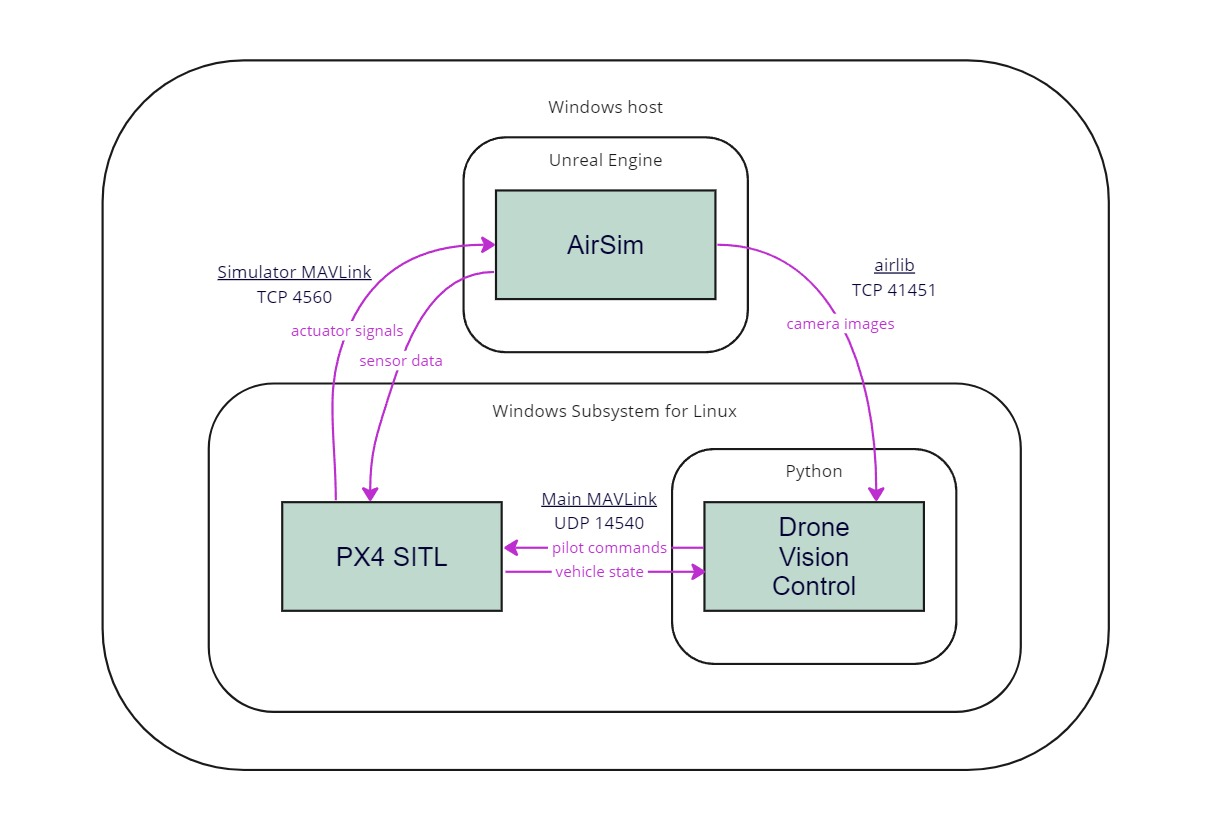
\includegraphics[width=0.8\textwidth,keepaspectratio]{img/sitl-connections.jpg}
  \caption{Connection diagram of how the three systems interact with each other during SITL simulation.}
  \label{fig:sitl-connections}
\end{figure}

The whole set of connections established in the software-in-the-loop simulation is shown in figure \ref{fig:sitl-connections} at the transport layer level.
The two systems that run inside the virtualized Linux system through WSL (the simulated flight stack and the Dronecontrol program) connect through the localhost network on the defined UDP port, and each of them connects in turn to the AirSim simulator through the virtual Local Area Network established by the Windows Subsystem for Linux to the host Windows computer.
The PX4 flight stack on SITL mode connects to the simulator using the TCP port 4560, as defined by PX4 on figure \ref{fig:px4-ports}, and Dronecontrol connects through the AirSim library \texttt{airlib}, which uses by default a TCP connection on port 41451.

In the case of hardware-in-the-loop simulation, the main difference with SITL is that the flight stack firmware runs on a physical flight board using a particular configuration.
In HITL, all motors/actuators are blocked, but internal software is fully operational.
This configuration adds another isolated system, so to simplify this mode of testing, since the WSL environment is no longer needed to run the flight stack, it is possible to move the execution of the Python modules to Windows.
This eliminates the need for additional configuration to allow the external flight controller to communicate with the internal WSL network, which is isolated by default from all external USB devices.
Furthermore, now that PX4 runs on a separate piece of hardware, it is necessary to establish a separate physical connection to the testing computer for each desired MAVLink channel,
either wired, through the micro USB port or an unused telemetry port on the flight controller, or wireless, through a telemetry radio.
Then both the simulator and the Python app can communicate with the flight controller independently.

\begin{figure}
  \centering
  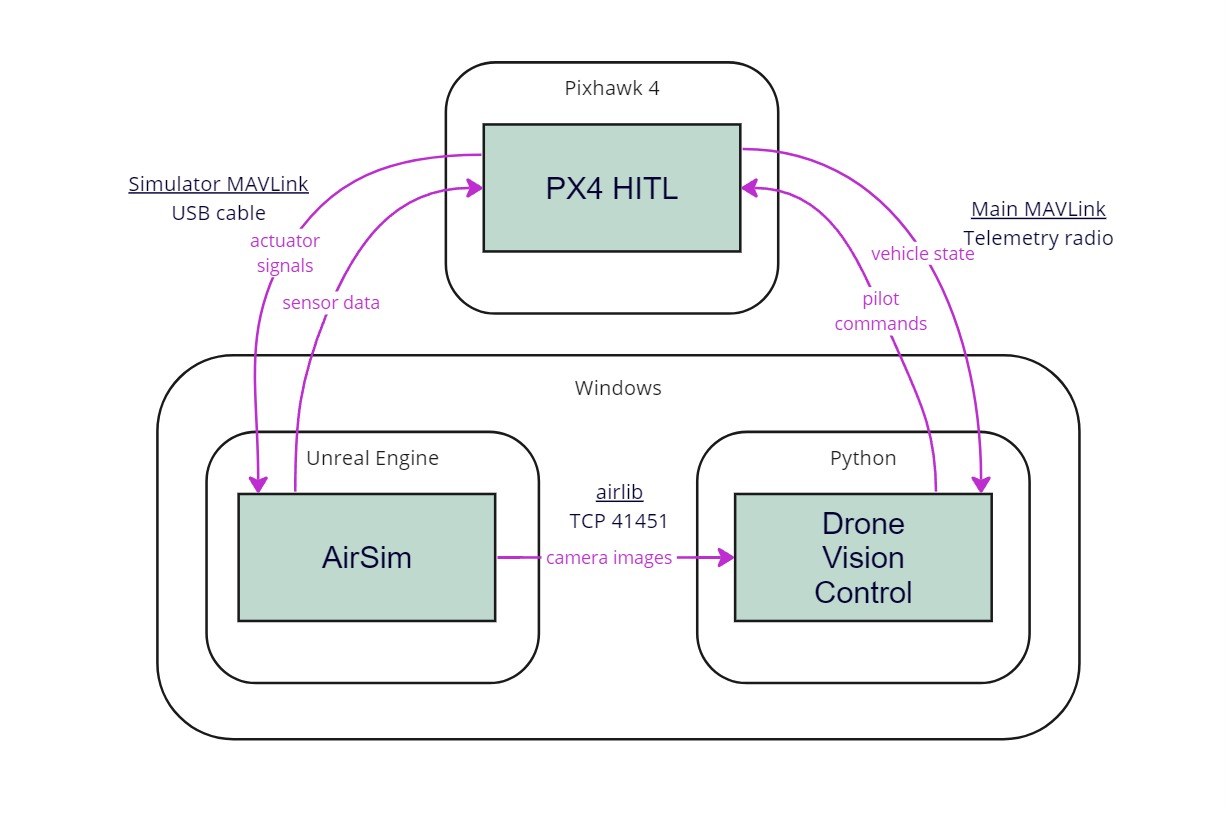
\includegraphics[width=0.8\textwidth,keepaspectratio]{img/hitl-connections.jpg}
  \caption{Connection diagram of how the three systems interact with each other during HITL simulation.}\label{fig:hitl-connections}
\end{figure}

Figure \ref{fig:hitl-connections} shows the chosen connections to execute tests in HITL mode.
The Windows machine runs both AirSim in Unreal Engine and Dronecontrol through the Python interpreter.
They communicate through TCP in the \texttt{localhost} network.
The board running PX4 connects to the simulator through a USB to micro USB cable, which is set up to work with a baudrate of 115200, and to the Python program through a telemetry radio running at a baudrate of 57600, both attached to USB ports on the Windows computer accessible through their COM address.

\subsubsection{AirSim testing environment}

Unreal Engine is a complex computer graphics generation program.
A project in the engine is defined through environments where components like 3D models, cameras, and lighting can be added.
AirSim is a plugin made for this engine by Microsoft, and although it also has released a version for the other most extended game engine in the market, Unity, it is experimental and limited in features.
The documentation contains all the necessary steps to get Unreal Engine and AirSim running on a Windows, Linux, or macOS operating system. 
However, Windows is the recommended environment \cite{build-airsim}.
The source code for the AirSim project includes a built-in Unreal environment that can be used to run tests and contains several 3D shapes like blocks and spheres, as well as a default quadcopter to act as the control vehicle.
It is also possible to create custom Unreal environments and run AirSim inside them by adding the built plugin and a custom vehicle to the project.

The environment used in this project for testing the Dronecontrol application is derived from the built-in AirSim environment and can be found on the project's repository \footnote{\url{https://github.com/l-gonz/tfg-giaa-dronecontrol/tree/main/AirSim}}.
It contains the default quadcopter vehicle, which includes several virtual cameras in order to be able to retrieve images from the vehicle's point of view in the simulated world, with some modifications to the background shapes and colours to provide better contrast to the camera.
The main addition to the environment is the 3D model of a human figure, to be used for testing the pose detection and tracking mechanisms in the computer vision solution.
This model is part of a free asset library of human models made by Renderpeople \cite{render-people} obtained from the Unreal Marketplace.
Figure \ref{fig:unreal-env} shows an image of the testing environment.
\todo[inline]{Add here if any additional changes to AirSim environment}


\begin{figure}
  \centering
  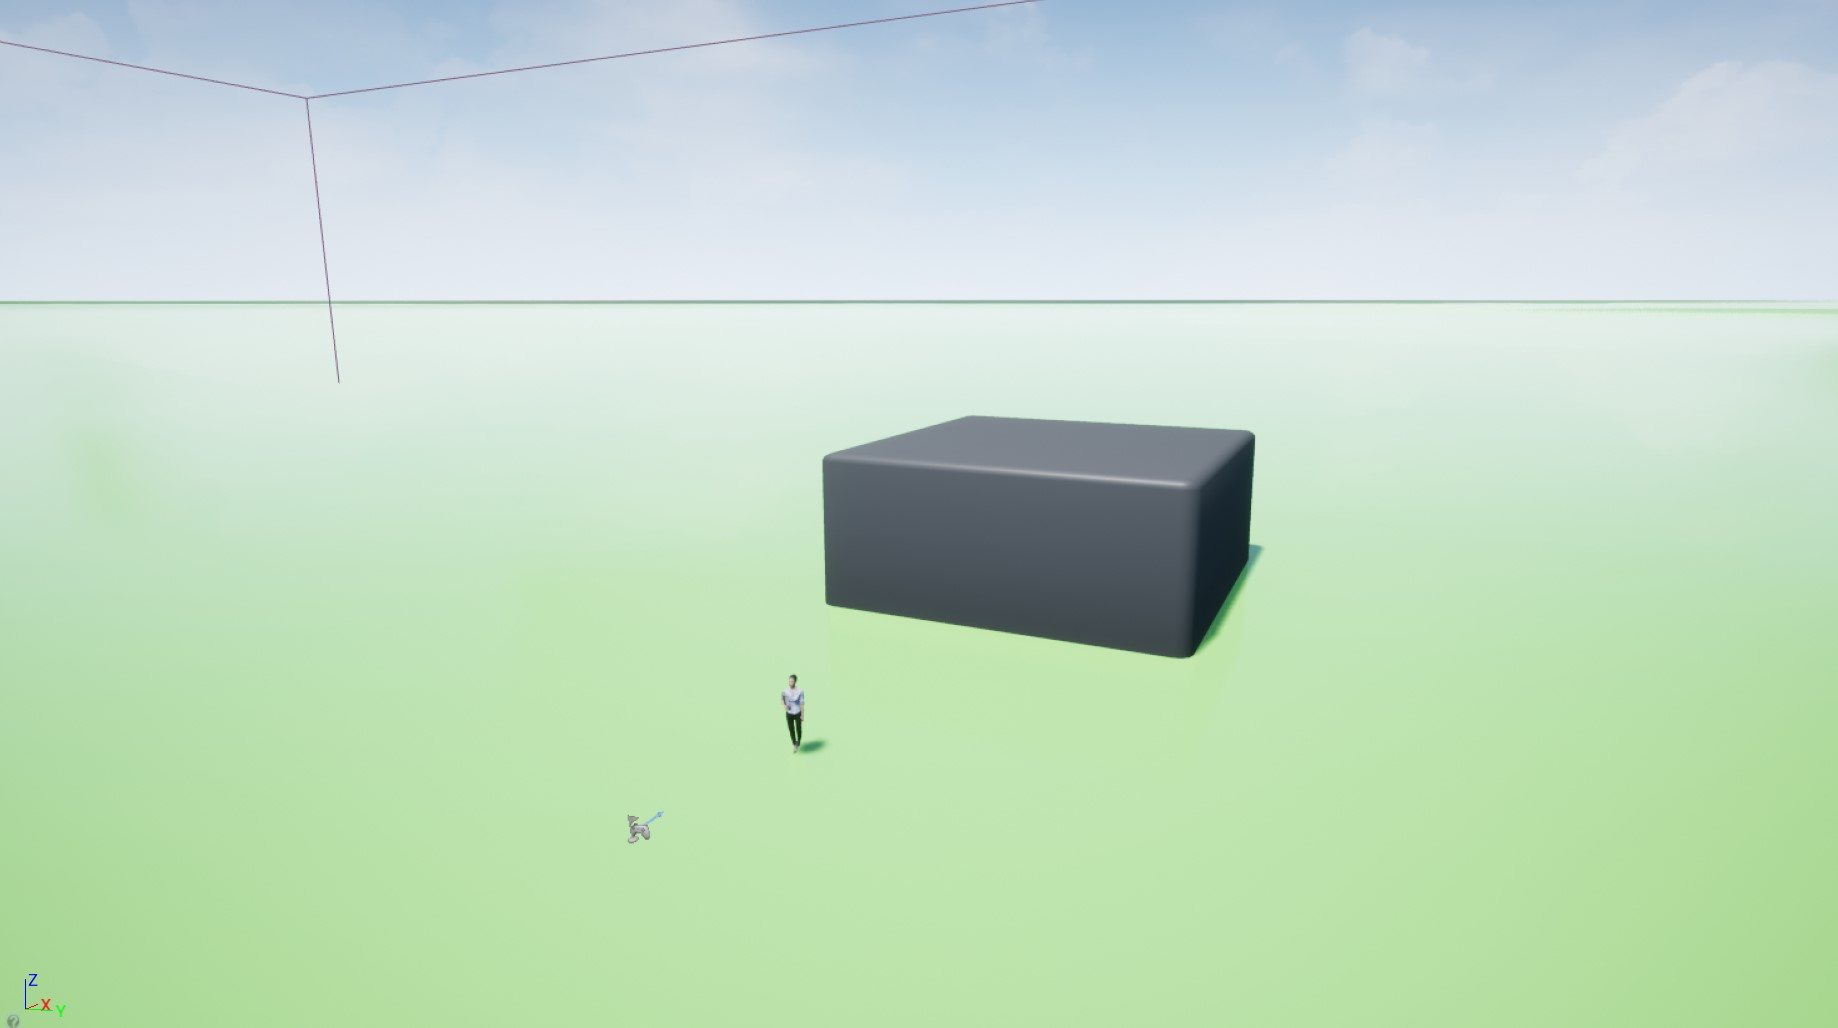
\includegraphics[width=\textwidth,keepaspectratio]{img/unreal-env.jpg}
  \caption{Screenshot from the Unreal Engine environment used for testing the computer vision solutions.}
  \label{fig:unreal-env}
\end{figure}


AirSim is compatible with both SITL and HITL simulation modes.
However, it must be set up to work with an external PX4 flight controller instead of AirSim's own internal \texttt{SimpleFlight} flight stack.
Appendix \ref{app:airsim-config} contains the required settings file for configuring these modes in AirSim,
where the \emph{"LocalHostIp"} needs to be exchanged with the IP of the Windows host in the local \texttt{vEthernet (WSL)} network to be able to connect between the simulator in Windows and the flight controller inside WSL.
This process is detailed further in the AirSim documentation \cite{airsim-doc-wsl} and in appendix \ref{app:install-airsim}.
In brief, the Unreal project with AirSim must first be set into play mode, and then the PX4 SITL flight controller must be built and started to attach to an already running simulator.
Inside the project in WSL, the flight controller can be run with all the necessary configuration for AirSim by using the provided shortcut script \footnote{\url{https://github.com/l-gonz/tfg-giaa-dronecontrol/blob/main/simulator.sh}}:
\begin{minted}{bash}
./simulator.sh --airsim
\end{minted}
Once the simulator and the flight controller are connected, an RC controller or QGroundControl can be used to control the vehicle, and other offboard applications like Dronecontrol can be attached to send any desired MAVLink commands.

For HITL, the \emph{"UseSerial"} setting should be set to true in the AirSim configuration, and the Pixhawk board should be connected to a USB port in the computer.
Additionally, the board should be set to HITL mode enabled from the QGroundControl safety configuration.
Then, the simulator will attach automatically to the board after starting play mode in Unreal.
Once the simulation has started, there is no noticeable change between the simulated flight controller in WSL (SITL mode) and the one running in the physical board (HITL mode).
